\documentclass [a4paper, 12pt]{article}

\usepackage{amssymb}
\usepackage{epsfig}
\usepackage{times}
\usepackage{float}
\usepackage[usenames,dvipsnames]{color}
\usepackage{ragged2e}
\usepackage[round,sort&compress]{natbib} 
\usepackage{multicol}
\usepackage{pgfgantt}
\usepackage{hyperref}
\usepackage{graphicx}
\usepackage{subcaption}
\usepackage[ddmmyyyy]{datetime}
\setlength\columnsep{6cm}
\usepackage[top=2cm, bottom=2cm, left=2cm, right=2cm]{geometry}
\setlength{\headsep}{1cm}
\setlength{\footskip}{1cm}
\setlength{\parindent}{1cm}

\setlength{\bibsep}{-2pt}

\def\LCDM{\mbox{$\Lambda$CDM}}
\def\kms{\rm km\ s^{-1}}
\def\hkpc{\mbox{$\rm h^{-1}$kpc}}
\def\hMpc{\mbox{$\rm h^{-1}$Mpc}}
\def\hGpc{\mbox{$\rm h^{-1}$Gpc}}
\def\hMsun{\mbox{$\rm h^{-1}$M$_\odot$}}
\def\lesssim{_ <\atop{^\sim}}
\def\gtsim{_ >\atop{^\sim}}


\newcommand{\aladin}{{\textsc{A}{ladin}}}
\newcommand{\topcat}{{\textsc{Topcat}}}
\newcommand{\cassis}{{\textsc{Cassis}}}
\newcommand{\simbad}{{\textsc{SIMBAD}}}
\newcommand{\vizier}{{\textsc{v}izie\textsc{r}}}
\renewcommand{\dateseparator}{.}
\newcommand{\datatree}{\textsc{Data Tree}}

\renewcommand\UrlFont{\color{blue}\rmfamily}

\begin{document}

\begin{center}
\includegraphics[width=0.3\textwidth]{../images/logo_euro.png} 
\hspace{5cm}
\includegraphics[width=0.4 
\textwidth]{../images/logo_asterics.png}\\
\vspace{1.5cm}
\begin{Huge} \textbf{ASTERICS - H2020 - 653477} \end{Huge} \end{center}

 
 \vspace{1cm}
\Huge
\begin{center}
\bf Abell 1656: the Coma\\ Cluster of Galaxies
  \end{center}

 
\vspace{1cm}
\large
\begin{center}
Massimo Ramella \& Giulia Iafrate\\ %Giulia Iafrate
\textit{INAF - Osservatorio Astronomico di Trieste}
\end{center}
\vspace{0.5cm}
\begin{center}
Caroline Bot \& Thomas Boch\\
\textit{updated for the doctoral day in Paris}\\
\vspace{0.5cm}
Jenny G. Sorce\\
\textit{updated with the new template for ASTERICS \& new plots}\\
\vspace{0.5cm}
Katharina A. Lutz\\
\textit{updated to \aladin\ v10}
\end{center}
\vspace{0.5cm}
\begin{center}
last update \today
\end{center}


\vspace{3.5cm}
Template by Jenny G. Sorce


\newpage
\normalsize
\vfill
\tableofcontents
\vfill

\newpage

\justify
\section{Introduction}

Goal: 
\begin{itemize}
\item  Examine the Coma cluster of galaxies (Abell 1656) using VO data and tools in order to perform a quick evaluation of the mean redshift and velocity dispersion of the cluster. 
\item Use redshifts and photometry (Petrosian r magnitude) of the SDSS survey and then add redshifts of the CAIRNS survey (Rines et al. 2003) in order to improve the completeness of the redshift sample. 
\item Look for hydrogen lines in HST spectra in the direction of this cluster and check whether the lines are consistent with foreground or with galaxy velocities.\\
\end{itemize}
\noindent The software packages we require to tackle these tasks are \aladin, 
\topcat\ and \cassis.

\section{Display the region of Abell 1656 in \aladin}
\label{sec:display}
\begin{itemize}
\item Launch \aladin: Open a terminal and type: \texttt{java -jar Aladin.jar 
\&}.
\item In \aladin, enter `A1656' (Coma Cluster) in the \textbf{Command} slot of 
the main window. \\
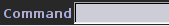
\includegraphics[width=0.2 \textwidth]{../images/aladin_command_empty.png}
\item Zoom/unzoom to work with galaxies in a region of about 40 by 40\,arcmin 
around the Coma cluster. At the distance of Coma, 40\,arcmin corresponds to 
1.1\,Mpc (with H$_0$=71~$\kms$~Mpc$^{-1}$, $\Omega_\Lambda$=0.73 and 
$\Omega_m$=0.27), a region large enough for our purposes. Tip: 
The cyan/blue numbers at the bottom of the main viewing window and in the 
overview panel in the bottom right corner of \aladin\ indicate the area shown 
in the main viewing window (Figure~\ref{fig:aladinA1656}). As a second option 
draw a 40' long arrow with the 
\textbf{dist} button 
\includegraphics[width=0.03  
\textwidth]{../images/aladin_button_distance.png}. 
\end{itemize}


\begin{figure}[H]
\center
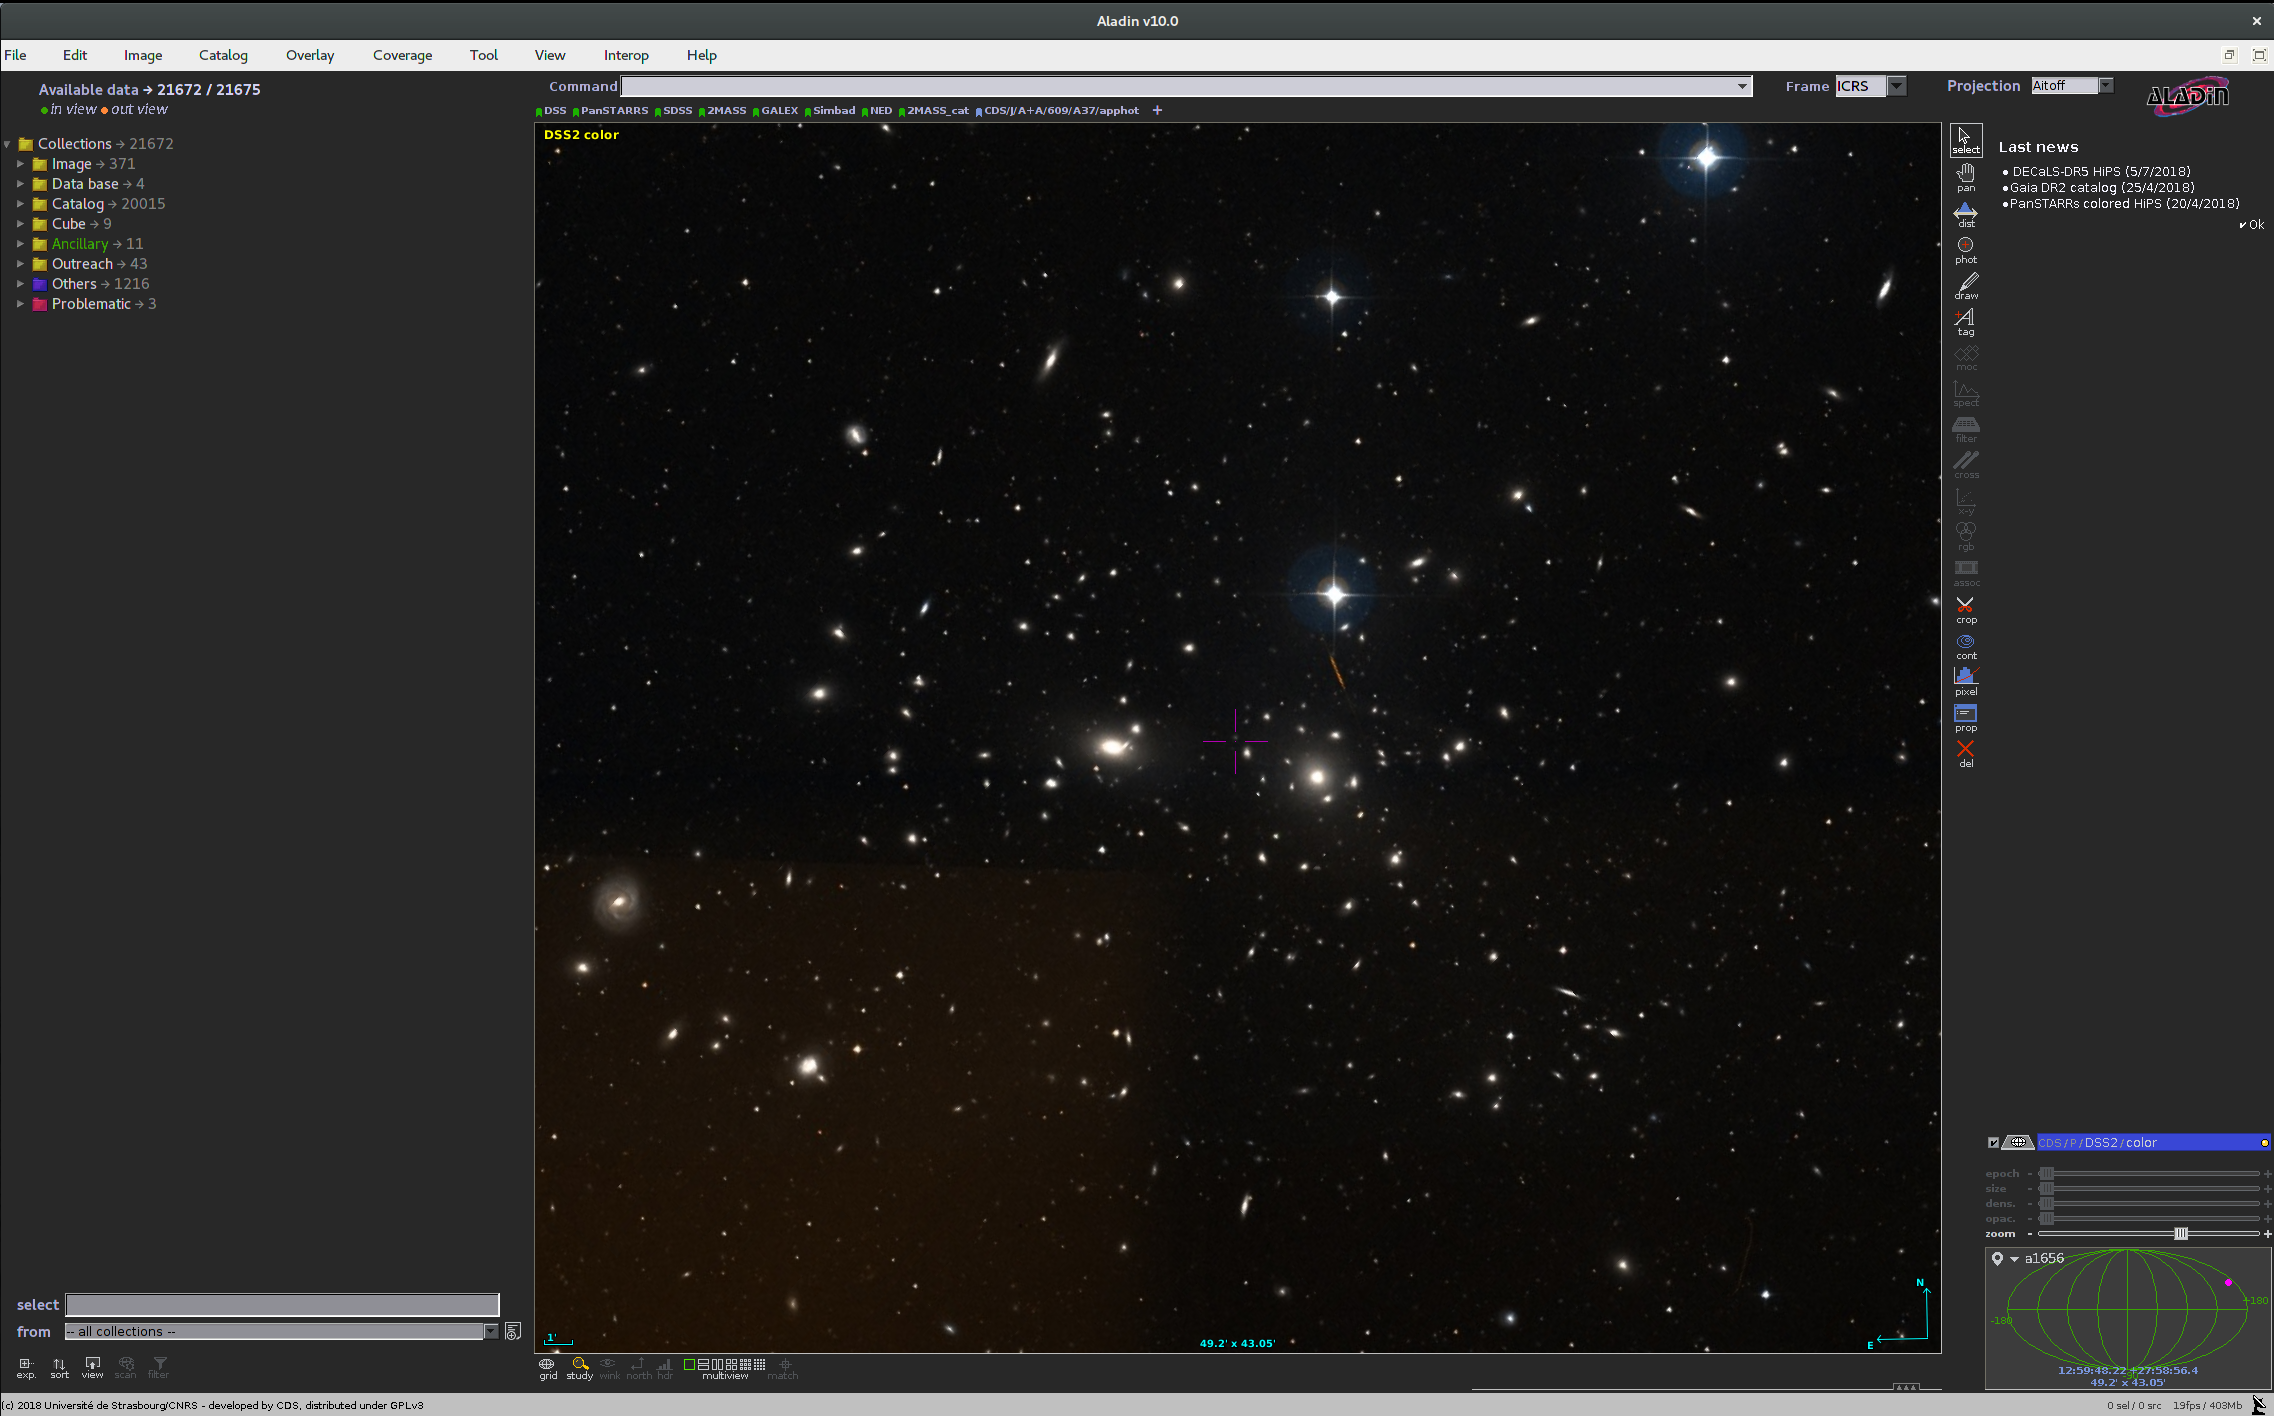
\includegraphics[width=0.85 \textwidth]{../images/aladin_a1656_new.png}
\caption{Abell 1656 (Coma Cluster) in \aladin}
\label{fig:aladinA1656}
\end{figure}

\section{Load the SDSS-DR9 catalogue and select galaxies}

\begin{itemize}
\item Load the SDSS-DR9 catalogue through the \datatree: Type "SDSS" in the 
\textbf{Select} line below the \datatree\ to limit the resources shown in the 
\datatree\ to those connected to SDSS 
\includegraphics[width=0.2 
\textwidth]{../images/aladin_select_SDSS.png}. You can further narrow down your 
search by restricting the collection of data sets with \textbf{from}  

\includegraphics[width=0.2 
\textwidth]{../images/aladin_selectfrom_largecatalogues.png}. More complex 
filters can be created by clicking on 
\includegraphics[width=0.03 
\textwidth]{../images/aladin_button_filtertree.png}. Under "Catalog" 
$\rightarrow$ "VizieR" $\rightarrow$ "II-Photometric Data" click on SDSS-DR8, 
make sure that the \textbf{in view} box is ticked 
\includegraphics[width=0.07 
\textwidth]{../images/aladin_load_inview.png} and click \textbf{Load} 
(Figure~\ref{fig:aladinSDSS}).

\begin{figure}[H]
\center
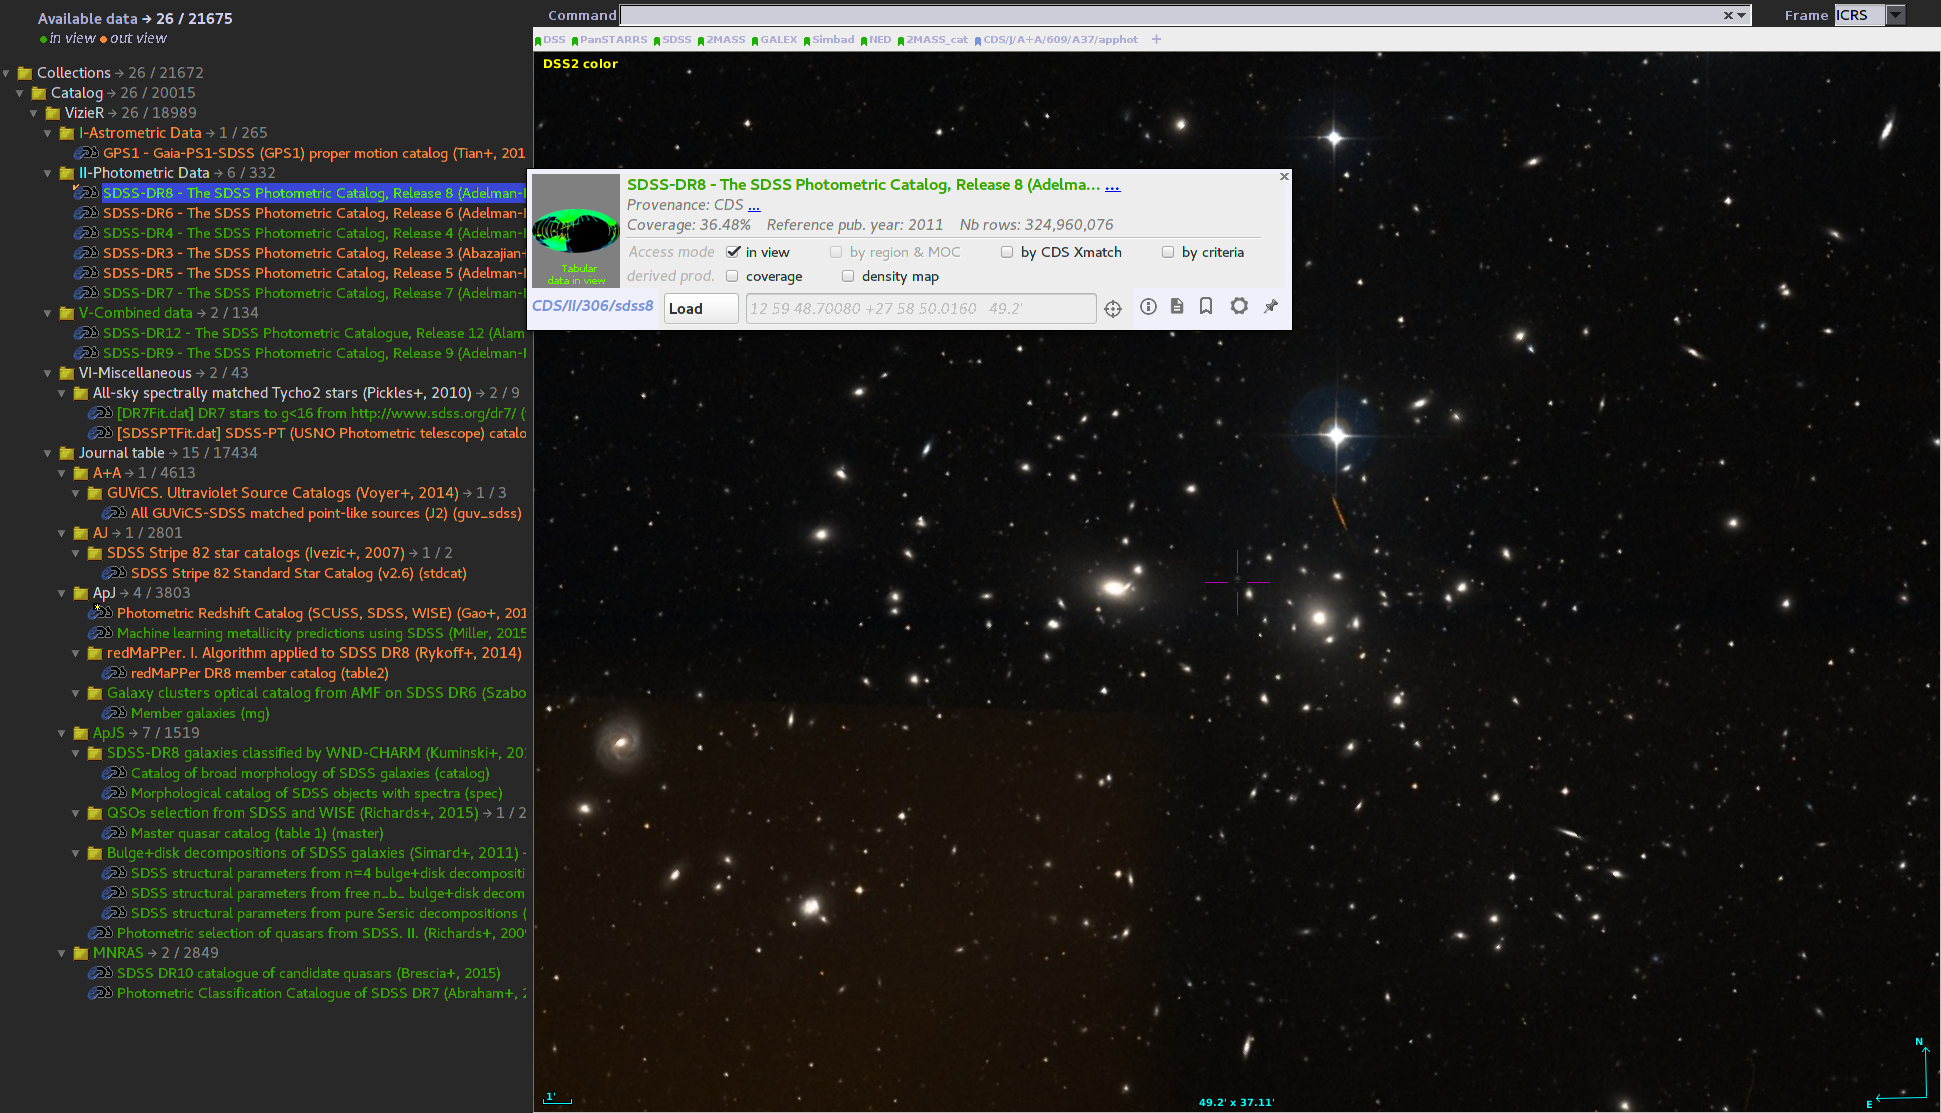
\includegraphics[width=0.85  
\textwidth]{../images/aladin_load_sdss_a1656.png}
\caption{The \aladin\ \datatree\ when filtered to "SDSS" resources in "large 
catalogues". Green resources have entries in the area of the sky that is 
currently shown in the main viewing window, orange ones not. The grey pop-up 
window allows you to load the data in different ways, e.\,g. load all data 
within the field of view or filter the catalogue by MOC. }
\label{fig:aladinSDSS}
\end{figure}

\item Catalogue data of approximately 50,000 sources have now been loaded. To 
limit this sample to galaxies (cl=3) that are also SDSS primary sources 
(mode=1) we continue as follows (Figure~\ref{fig:aladinfilter}):
\begin{itemize}
    \item In the \aladin\ stack (right), select the catalogue plane, click on 
    the \textbf{Filter} button  
\includegraphics[width=0.04  
    \textwidth]{../images/aladin_button_filter.png} and write the following 
    syntax in the \textbf{Advanced mode} tab: \newline
    \texttt{\$\{cl\}=3\&\&\$\{mode\}=1\{draw\}} \newline
    Clicking \textbf{Apply} ensures that our sample is selected according to 
    our selection criteria and that only sources that adhere to these criteria 
    are shown in the main viewing window. 
    \item Still in the filter window, clicking \textbf{Export} will build a new 
    plane with only filtered sources included.
    \item Note that the \textbf{Pick} line above the free syntax field is 
    helpful to create other filters.
\end{itemize}

\begin{figure}[H]
\center
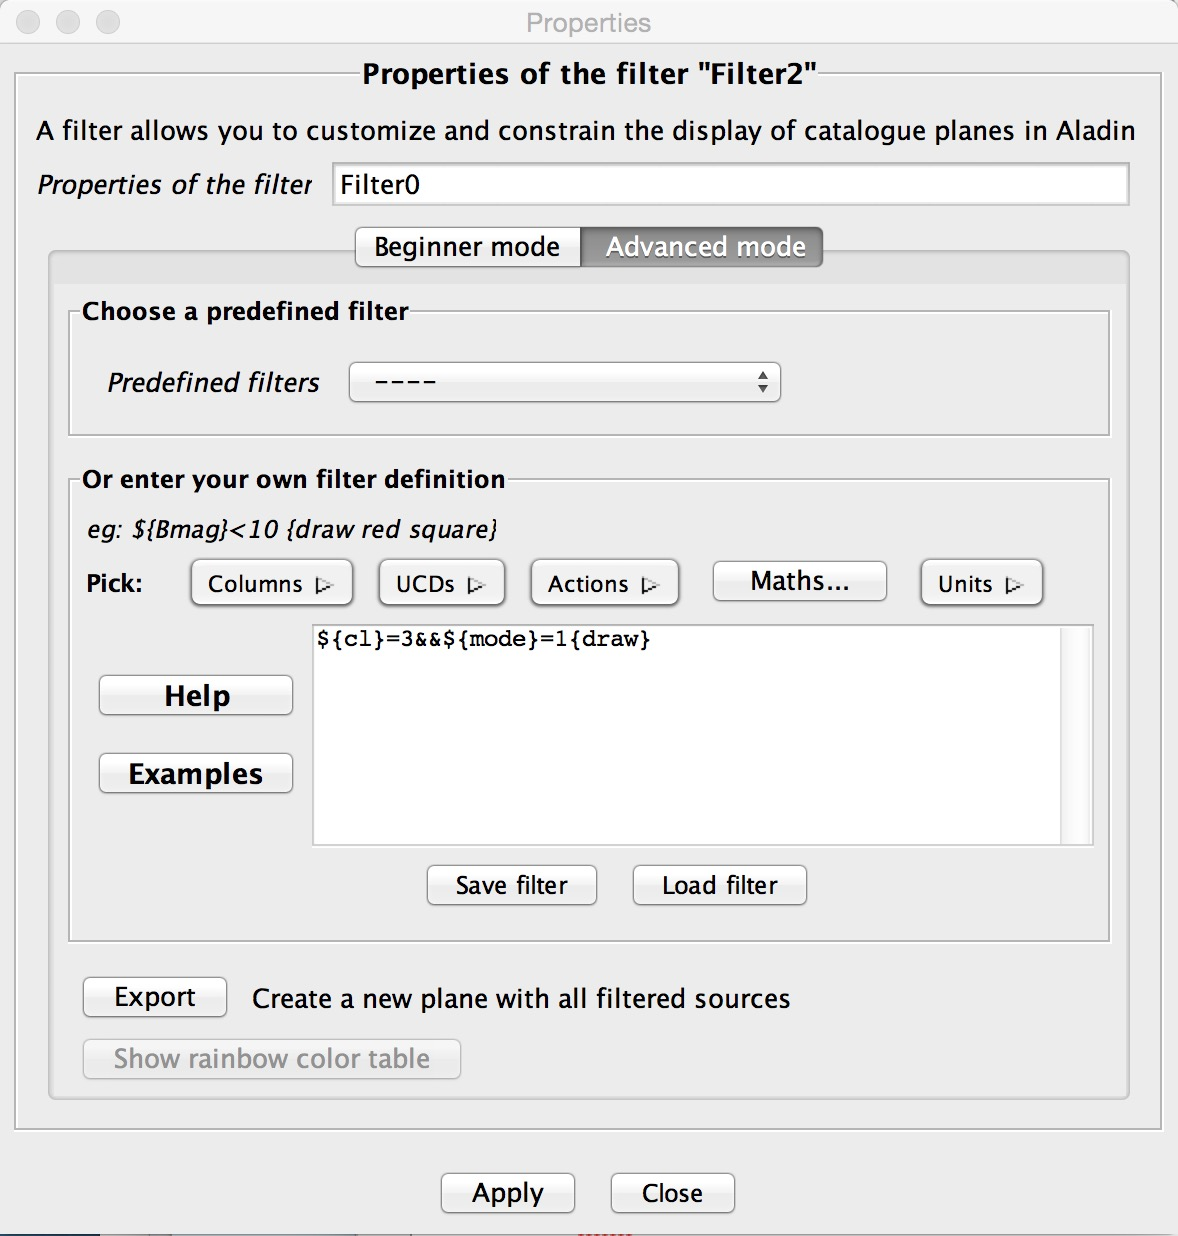
\includegraphics[width=0.4\textwidth]{../images/aladin_filter_galaxies-sdss.jpg}
\caption{Filtering with \aladin}
\label{fig:aladinfilter}
\end{figure}

\item Rename this new plane SDSSgalaxies using the \textbf{Properties} button  

\includegraphics[width=0.03
\textwidth]{../images/aladin_button_properties.png}. Depending on your field of 
view the new filtered catalogue includes around 35,000 sources.

\item Broadcast the filtered catalogue to \topcat. You can do so by 
right-clicking on the catalogue plane and selecting \textbf{Broadcast selected 
tables to...$>$ topcat}. Beware that \topcat\ must be launched for this 
function to be enabled.  

\begin{figure}[H]
\center
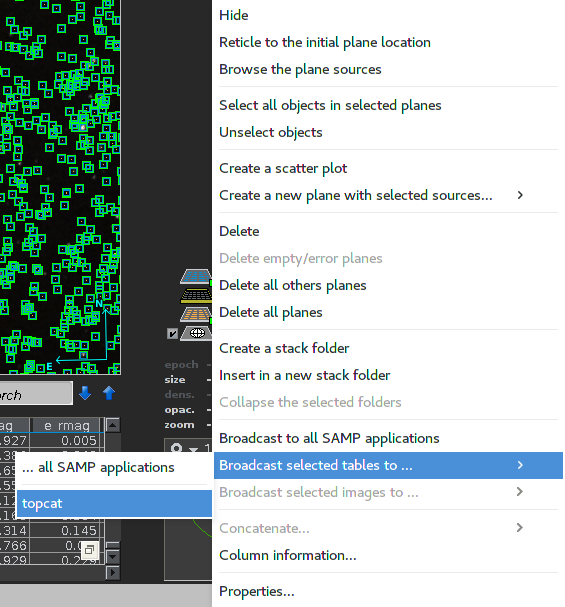
\includegraphics[width=0.4 \textwidth]{../images/aladin_send_table_topcat.png}
\caption{Broadcasting the filtered catalogue to \topcat.}
\label{fig:topcatbroadcast}
\end{figure}

\item In \topcat, display the column metadata with 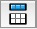
\includegraphics[width=0.04  
\textwidth]{../images/topcat_button_metadata.jpg}. In the new window, deselect 
all rows    
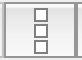
\includegraphics[width=0.04  \textwidth]{../images/topcat_button_invisible.jpg} 
and then select  
\includegraphics[width=0.04  
\textwidth]{../images/topcat_button_select.jpg} 
only the four necessary columns: RA\_ICRS (\$10), DE\_ICRS (\$11), zsp (\$12) 
and rmag (\$17).
\end{itemize}

\section{Identify the brightest sources as being stars contaminating the sample}

\begin{itemize}
\item In the main \topcat\ window, open the subset window  
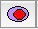
\includegraphics[width=0.04  \textwidth]{../images/topcat_button_subset.jpg} 
and build a subset of the brightest sources (with magnitudes rmag$<$11.5):
\begin{itemize}
    \item In the subset-window, click on 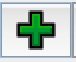
\includegraphics[width=0.04  
    \textwidth]{../images/topcat_button_add.jpg}  to define a new row subset.
    \item \textbf{Subset name}: `stars'.
    \item \textbf{Expression}: \texttt{\$17$<$11.5} or \texttt{rmag$<$11.5} 
    (Note: \topcat\ expressions 
    do not differentiate small/capital letters. Depending or the column names 
    of the table you might have to use \$ID of the column rather than its name. 
    \$ID can be found with \textbf{Views $\rightarrow$ Column Info} or 
    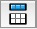
\includegraphics[width=0.04 
    \textwidth]{../images/topcat_button_metadata.jpg} in 
    the main \topcat\ window).
\end{itemize}
\item There are two options to check in \aladin\ that each source in the star 
subsample is indeed a star:
\begin{itemize}
    \item In the main \topcat\ window, select the `stars' subset of the 
    SDSSgalaxies catalogue  
\includegraphics[width=0.2  
    \textwidth]{../images/topcat_dropdown-menu_subsets.jpg} and broadcast it to 
    \aladin\ 
    (\textbf{Interop $\rightarrow$ Send table to $\rightarrow$ Aladin} or  
    
\includegraphics[width=0.04  
    \textwidth]{../images/topcat_button_broadcast.jpg}). Switch to 
    \aladin\ and look through the sources by clicking on their entry in the 
    table. Zoom/unzoom as necessary. 
    \item In \topcat\ go to \textbf{Views} $\rightarrow$ \textbf{Activation 
    Action} or 
\includegraphics[width=0.035  
    \textwidth]{../images/topcat_button_activationaction.png}. In the newly 
    opened window, tick the box of and select \textbf{Send Sky Coordinates}. 
    Upon selection you can edit the settings for this activation action. See 
    Figure~\ref{fig:topcat_activation} for the options chosen for our case. If 
    you now display the table cell data (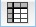
\includegraphics[width=0.035  
    \textwidth]{../images/topcat_button_open-tab.jpg}), you can click on any 
    table entry 
    and the corresponding source will be displayed in \aladin. Again 
    zoom/unzoom as necessary. 
\end{itemize}
\end{itemize}

\begin{figure}[H]
     \center
     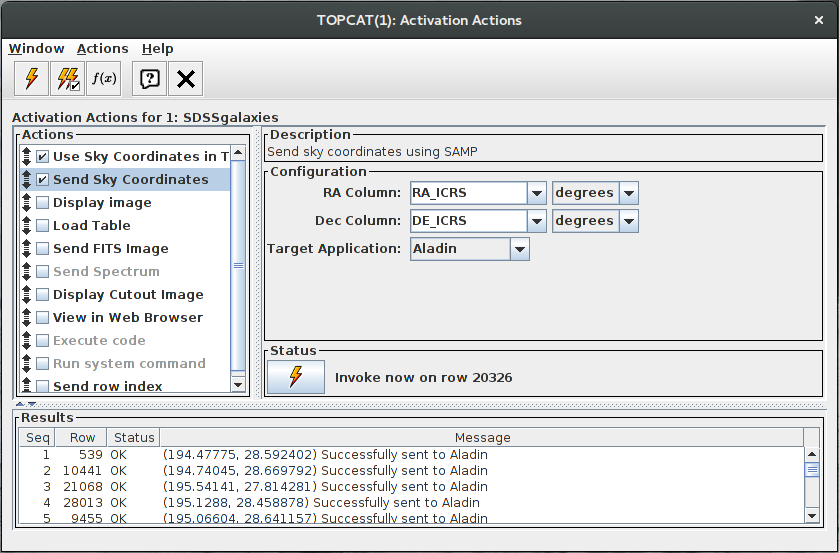
\includegraphics[width=0.6 
     \textwidth]{../images/topcat_window_activationaction.png}
     \caption{Setting up activation actions in \topcat.}
     \label{fig:topcat_activation}
\end{figure}

\section{Build a subset of galaxies with photometry (rmag) and redshift (zsp) 
in SDSS}

\begin{itemize}
\item In the main \topcat\ window, open the subset window  
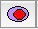
\includegraphics[width=0.04  \textwidth]{../images/topcat_button_subset.jpg} 
again and 
build a subset of galaxies (no stars, i.e. \texttt{rmag$>$11.5}) with magnitude 
rmag brighter than 17.77\,mag (completeness limit of the SDSS spectroscopic 
sample) and redshift information. This can be done with the subset expression: 
\texttt{zsp$>$0 \&\& rmag$<=$17.77 \&\& rmag$>$11.5}. Call this subset `zsp17'.
\item In the main window of \topcat\ select the subset `zsp17' and duplicate the table (\textbf{File $\rightarrow$ Duplicate Table}).
\item Rename the new table to `zsp17'. 
\end{itemize}


\section{Improve the completeness with other sources of redshifts in \vizier}

\begin{itemize}
\item In \topcat, build the subset `nozsp17' that contains galaxies with 
the same magnitude selection as before but no redshifts (use 
\texttt{!(zsp$>$0)} 
instead of \texttt{zsp$>$0} in the above expression). Again depending on your 
field of view the new subset contains between 100 and 200 entries.
\item Select the subset `nozsp17' in \topcat\ main window, duplicate the table and rename the new table `nozsp17'.
\item In \topcat\ main window, search optical catalogues with redshifts:
\begin{itemize}
    \item Go to \textbf{VO $\rightarrow$ \vizier\ catalogue service}.
    \item Select \textbf{Cone selection}: \textbf{Object name}=`A1656', click 
    on \textbf{resolve}, \textbf{radius}=`40'\,arcmin. Then select \textbf{All 
    Rows}.
    \item In the \textbf{catalogue selection} section: select the \textbf{by 
    Keywords} tab and enter `redshifts Rines', load the \textbf{Rines+ 2003} 
    catalogue. Two tables are loaded. Delete the cluster catalogue to keep only 
    the galaxy one (\textbf{File $\rightarrow$ Discard Table(s)}).
\end{itemize}

\begin{figure}[H]
\center
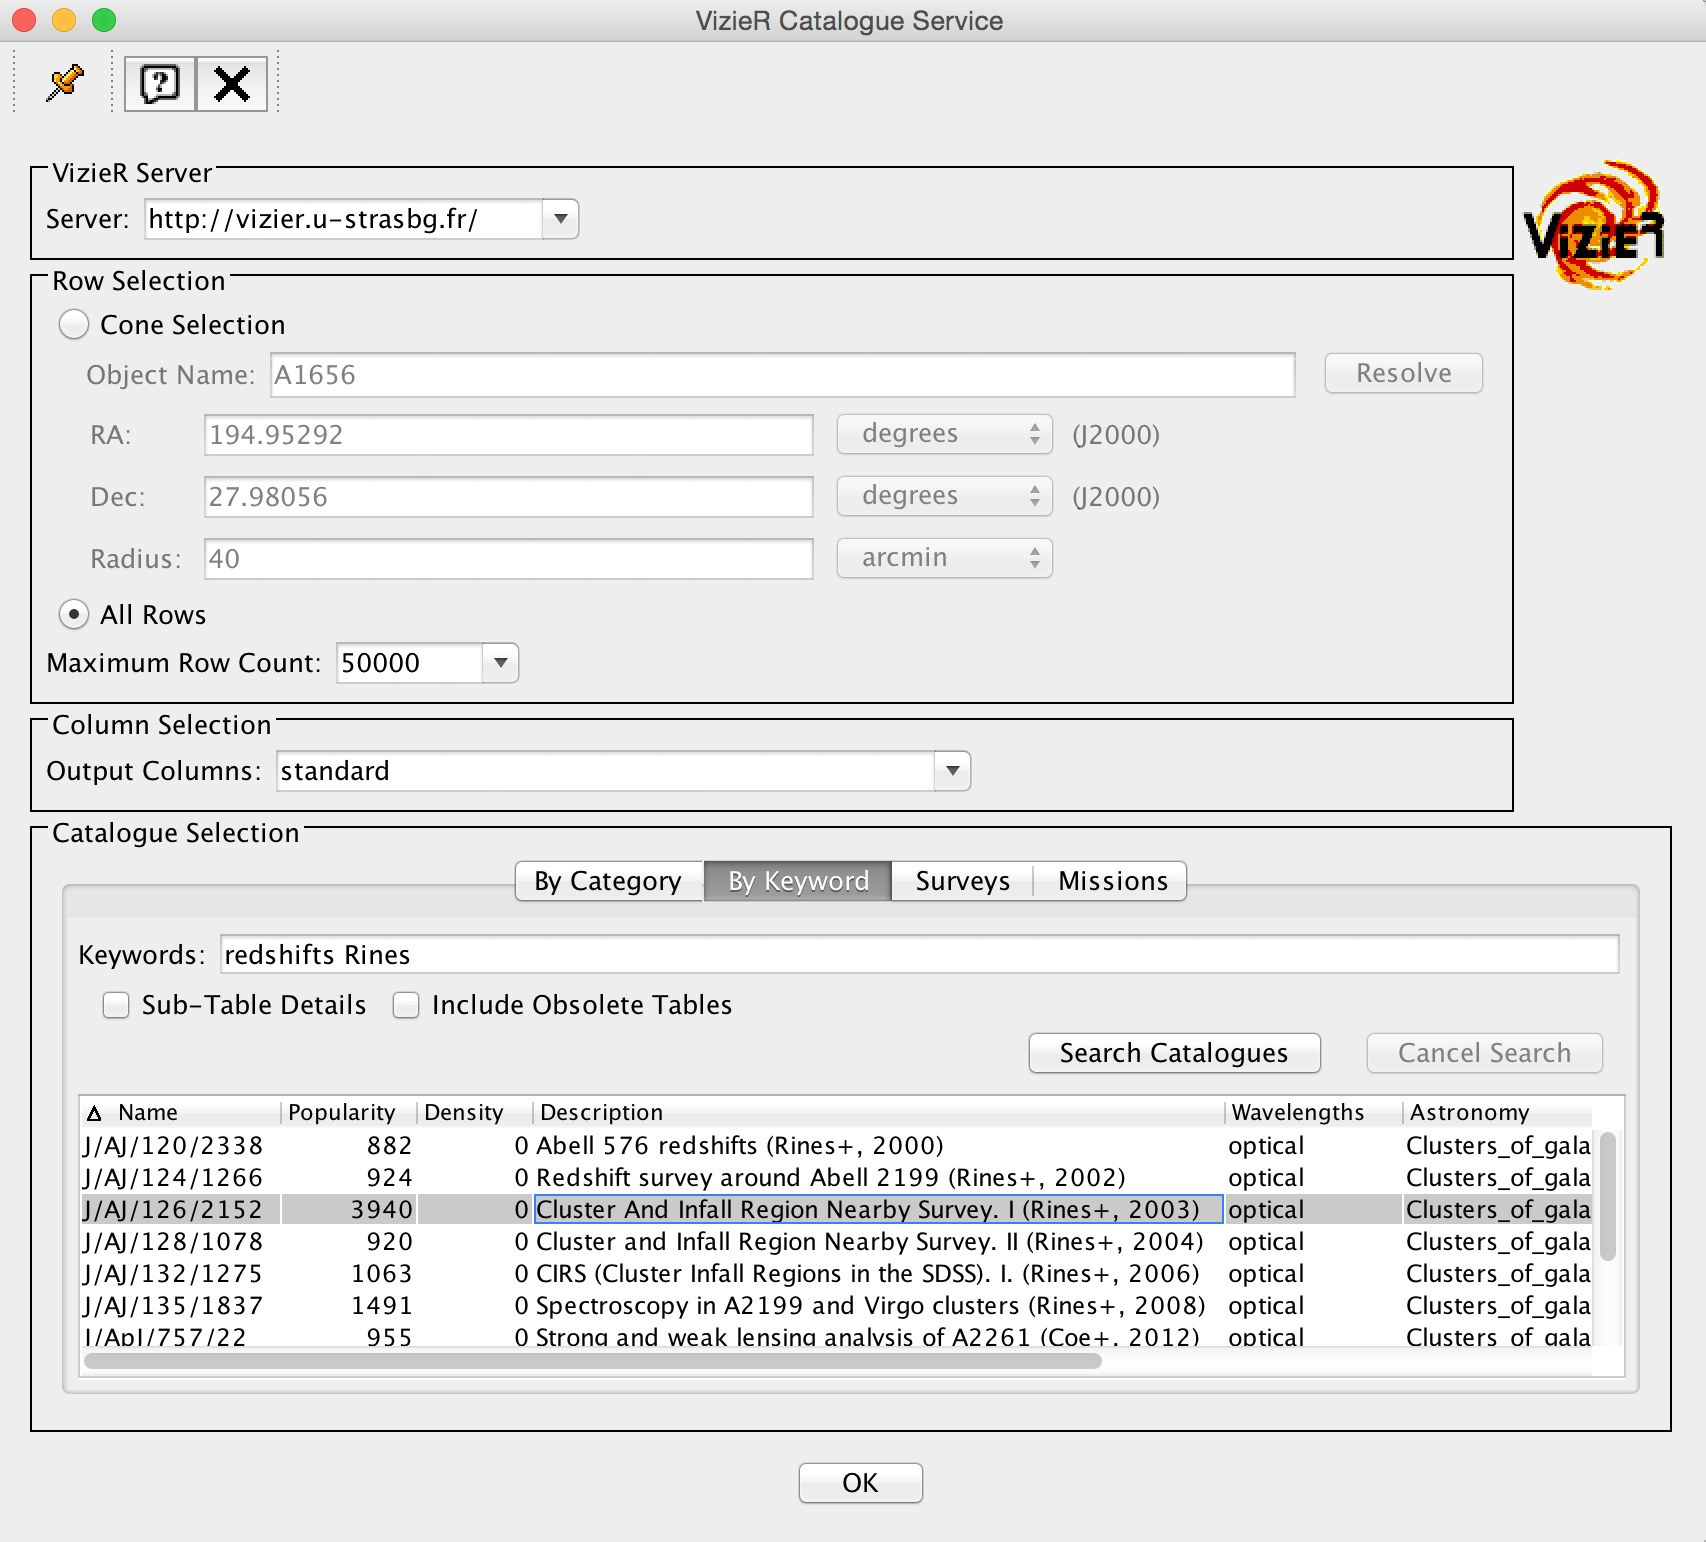
\includegraphics[width=0.5  \textwidth]{../images/topcat_vizier_rines2003.jpg}
\caption{Loading a catalogue from \vizier\ with \topcat.}
\label{fig:topcatvizier}
\end{figure}

\item Find redshifts in Rines+ catalogue for galaxies without redshift in 
nozsp17:
\begin{itemize}
    \item X-match the `nozsp17' and the Rines catalogue (\textbf{Joins 
    $\rightarrow$ pair match} or  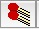
\includegraphics[width=0.04  
    \textwidth]{../images/topcat_button_xmatch.jpg})
    \item Use \textbf{sky} algorithm with `5\,arcsec' max error and choose 
    \textbf{Best match, symmetric}. See Figure~\ref{fig:topcatxmatch} for  more 
    details. 
\end{itemize}

\begin{figure}[H]
\center
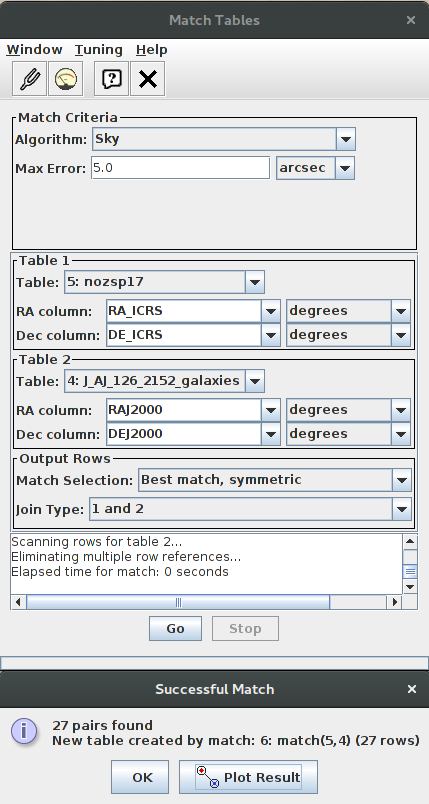
\includegraphics[width=0.3  
\textwidth]{../images/topcat_match_SDSS_Rines2003.png}
\caption{X-matching with \topcat.}
\label{fig:topcatxmatch}
\end{figure}
\end{itemize}

\section{Build the final catalogue including Rines+ redshifts}

\begin{itemize}
\item Add a new column to `zsp17' catalogue to get the apparent radial velocity 
cz:
\begin{itemize}
    \item Click \textbf{Table Columns}  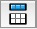
\includegraphics[width=0.04  
    \textwidth]{../images/topcat_button_metadata.jpg}, then do \textbf{Columns 
        $\rightarrow$ New Synthetic Column} or click  
        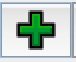
\includegraphics[width=0.04  
    \textwidth]{../images/topcat_button_add.jpg}.
    \item \textbf{Name}: `czsp'
    \item \textbf{Expression}: \texttt{toInteger(zsp*300000)}
\end{itemize}
\item Concatenate `zsp17' and match tables (\textbf{Joins $\rightarrow$ 
Concatenate Tables}). Fill in the \textbf{Appended Table} tabs. The final 
catalogue contains around to 700 galaxies.
\begin{figure}[H]
\center
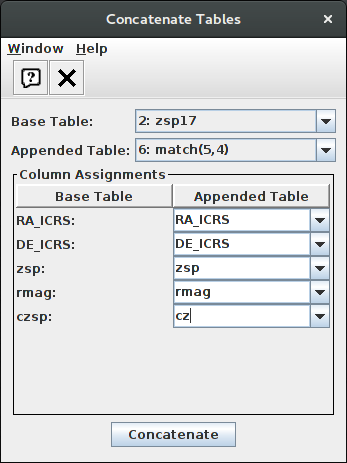
\includegraphics[width=0.3  
\textwidth]{../images/topcat_concatenate_SDSS_Rines2003.png}
\caption{Concatenating with \topcat.}
\label{fig:topcatconcat}
\end{figure}
\end{itemize}

\section{Determine the cz distribution, $<$cz$>$ and dispersion in \topcat}
\label{sec:det_cz}
\begin{itemize}
\item View the histogram of `czsp' values with  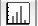
\includegraphics[width=0.06  
\textwidth]{../images/topcat_button_histogram.jpg}
\item Isolate the main peak of Coma in the histogram by selecting the 
appropriate region scrolling your mouse or playing with \textbf{Axes} 
(\textbf{Range} tab) and \textbf{Bins} (\textbf{Bin size})  
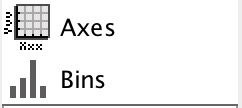
\includegraphics[width=0.1  \textwidth]{../images/topcat_set_axes-bins.jpg} 
(see Figure~\ref{fig:comapeak} for an example).
\begin{figure}[H]
\center
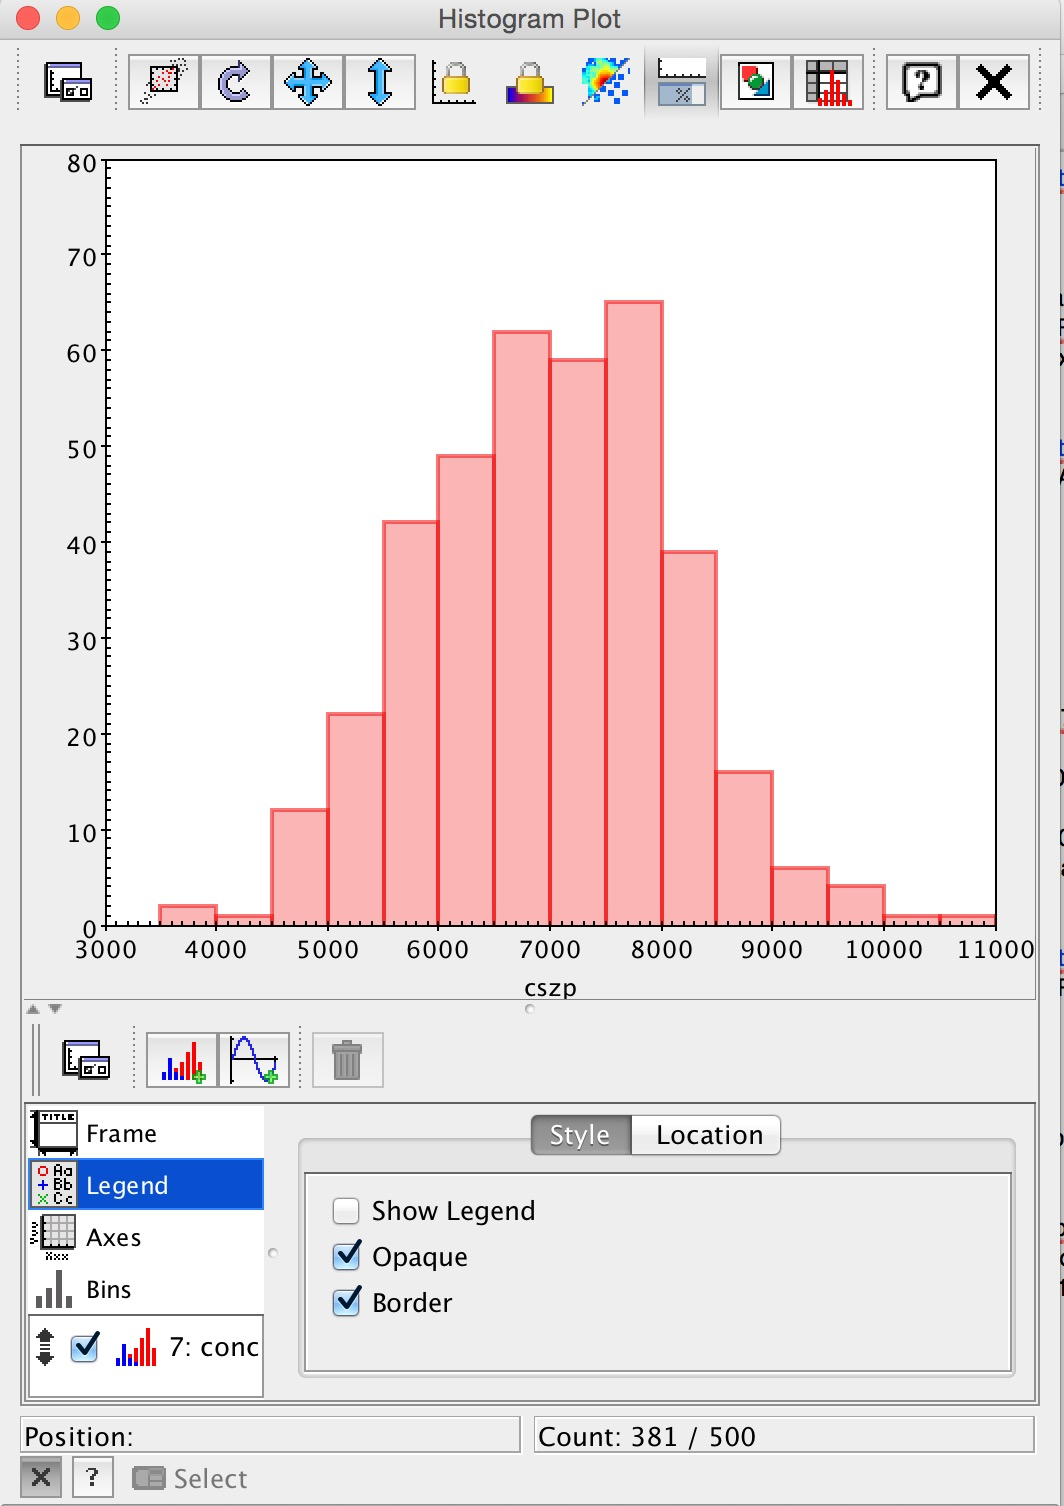
\includegraphics[width=0.33  \textwidth]{../images/topcat_coma-velo-peak.jpg}
\caption{Main peak of the Coma cluster.}
\label{fig:comapeak}
\end{figure}
\item Build a new subset named `Coma' using the range of cz observed in the 
histogram (proceed as before to build new subsets or once having zoomed in on 
the Coma peak use this button: 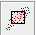
\includegraphics[width=0.03 
\textwidth]{../images/topcat_button_selection-plot.png} ).
\item Select this Coma subset in the main window of \topcat\ and open the 
\textbf{Row Statistics} window  
\includegraphics[width=0.04  
\textwidth]{../images/topcat_button_stats.jpg}. You will find something like 
$<$cz$>\approx$7000$\kms$ and SD$\approx$1000$\kms$ both in excellent agreement 
with more refined analyses (Figure~\ref{fig:topstats}). 
\begin{figure}[H]
\center
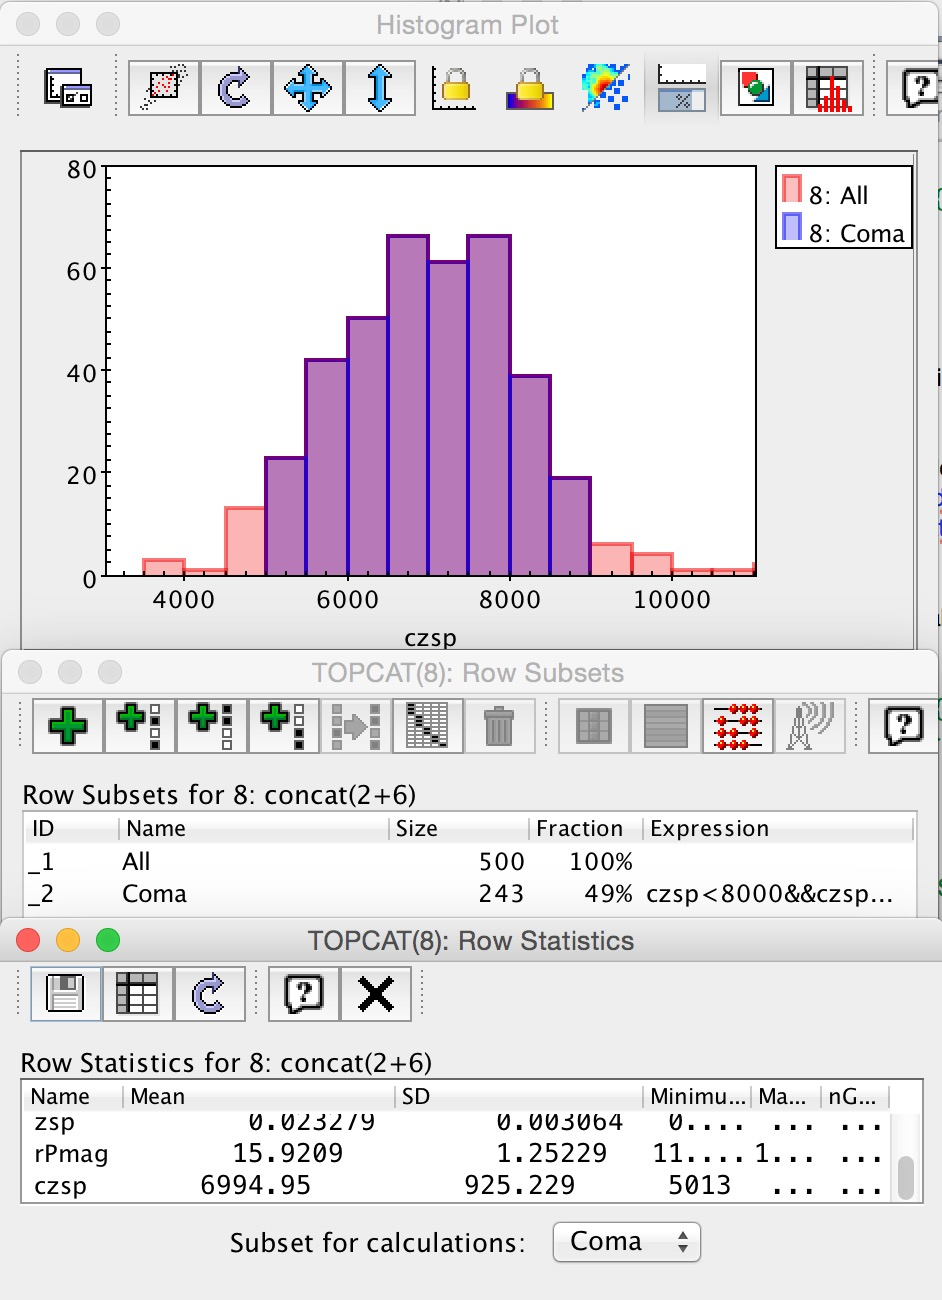
\includegraphics[width=0.33  \textwidth]{../images/topcat_hist-stat_coma.jpg}
\caption{Statistics with \topcat.}
\label{fig:topstats}
\end{figure}
\end{itemize}

\section{Look for HST spectra in the Coma Cluster}

\begin{itemize}
\item Go back to the \aladin\ window. Adjust the main viewing window such that 
once again it is centred on "A1656" and has a field of view of approximately 
$40\times40$\,arcmin. 
\item Type "HST" in the \textbf{Select} line and set \textbf{from} to "-\,-~all 
collections~-\,-". Narrow down the search in the Data discovery Tree filter 
window 
\includegraphics[width=0.03 
\textwidth]{../images/aladin_button_filtertree.png} by ticking the box of 
\textbf{SSA} (for Simple Spectral Access) in the \textbf{Technical} tab. 
\item Select \textbf{Others} $\rightarrow$ \textbf{SSA} $\rightarrow$ 
\textbf{mast.stsci} $\rightarrow$ \textbf{Hubble Space Telescope Spectra}, tick 
\textbf{in view} and then \textbf{Load} the table. 
\item Find the table entry for source 1257-2840 and (left-) click on the link 
in the url of the spectrum (in the first column). This will open an menu and 
allow you to broadcast the spectrum to \cassis\ (if \cassis\ is up and 
running). 
\end{itemize}
\begin{figure}[H]
    \center
    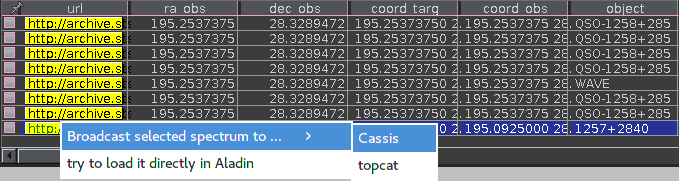
\includegraphics[width=0.6  
    \textwidth]{../images/aladin_send_HSTspec_cassis.png}
    \caption{Broadcast the spectrum of 1257-2840 to \cassis.}
    \label{fig:broadcastspectrum}
\end{figure}

\section{Visualize and analyse the HST spectrum with \cassis}

\begin{itemize}
\item Once the spectrum is transferred to \cassis, the \textbf{Spectrum 
Manager} appears. Select \textbf{Display Spectrum} 
\includegraphics[width=0.2  
\textwidth]{../images/cassis_button_display-spectrum.png}. The 
spectrum is now displayed in the \cassis\ main window. Two lines are clearly 
visible: one around 1250 Angstr\"om and one around 1350 Angstr\"om (see 
Figure~\ref{fig:spectrum}). 


\begin{figure}[H]
\center
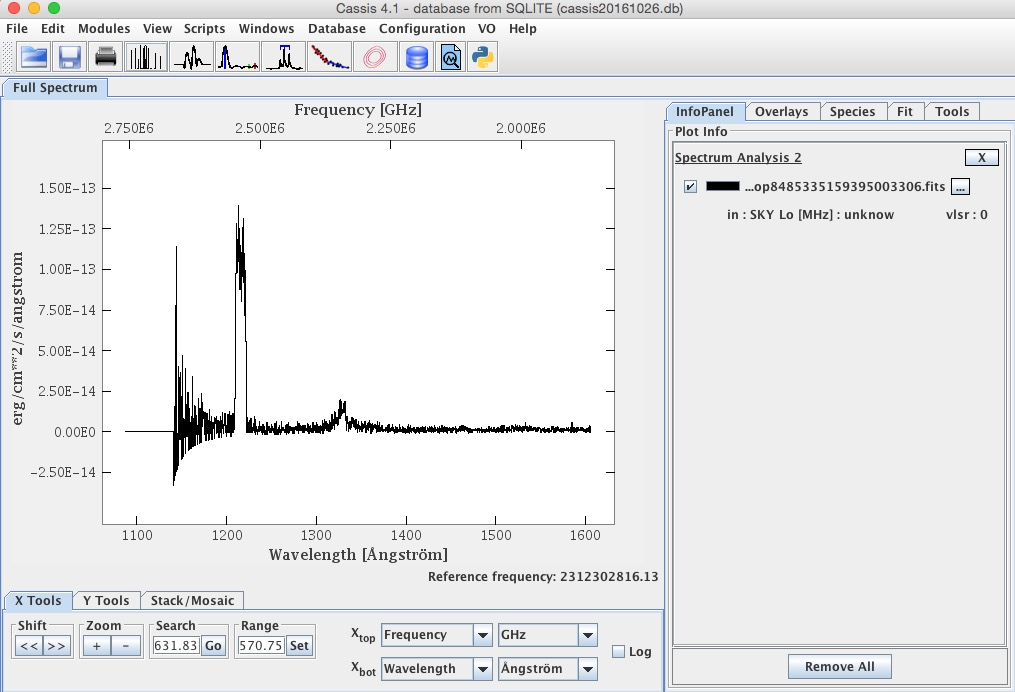
\includegraphics[width=0.6  \textwidth]{../images/cassis_display_spectrum-1.jpg}
\caption{Visualisation of the spectrum with \cassis.}
\label{fig:spectrum}
\end{figure}
\item To check that these are hydrogen lines (Ly$\alpha$), one at the local 
velocity, the other at the velocity of the Coma cluster 
(Figure~\ref{fig:spectrum2}):
\begin{itemize}
    \item Select the \textbf{Species} tab. Choose the \textbf{Full NIST} 
    database in the \textbf{Template} section.
    \item Unselect all species by clicking on the \textbf{Sel.} column.
    \item Select the sole \textbf{HI} line by ticking only this line.
    \item The maximum \textbf{Eup threshold} is by default too low for our 
    case. Remove the `150.0K' and replace it with ` *  ' to get all the HI 
    transitions without any threshold in energy.
    \item Tick \textbf{show signal} and click \textbf{Display} at the bottom of 
    the window. A green tick appears below the largest of the two lines. This 
    confirms that this line is an Hydrogen line at a zero velocity. Clicking on 
    the green tick gives more information on the line parameters. A right click 
    allows you to edit the overlay (useful for a copy-paste).
\end{itemize}

\begin{figure}[H]
\center
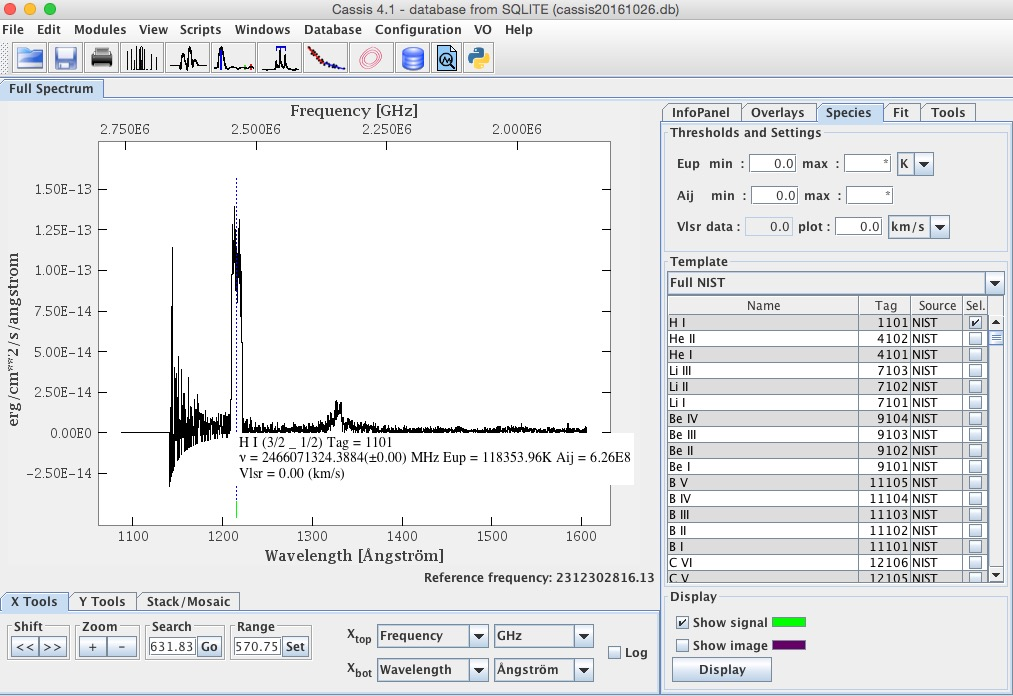
\includegraphics[width=0.6  \textwidth]{../images/cassis_display_spectrum-2.jpg}
\caption{Spectrum with \cassis. The the blue, dotted line and the green dash 
mark the location of the Ly$\alpha$ line at a line of sight velocity of 
0.0\,$\kms$}
\label{fig:spectrum2}
\end{figure}

\item To look for the LSR velocity of the galaxy in \simbad:
\begin{itemize}
\item Go back to the \aladin\ window and centre the image on the pointing 
centre of the HST spectral observations by double-clicking on the table row of 
the source 1257-2840. Zoom in or out as necessary. 
\item Make sure that the \textbf{Simbad Pointer} is activated (a tick next to 
\textbf{Tool} $\rightarrow$ \textbf{Simbad pointer}). 
\item Hover over of the pointing centre of the HST spectral observations until 
a small window appears. 
\begin{figure}[H]
\center
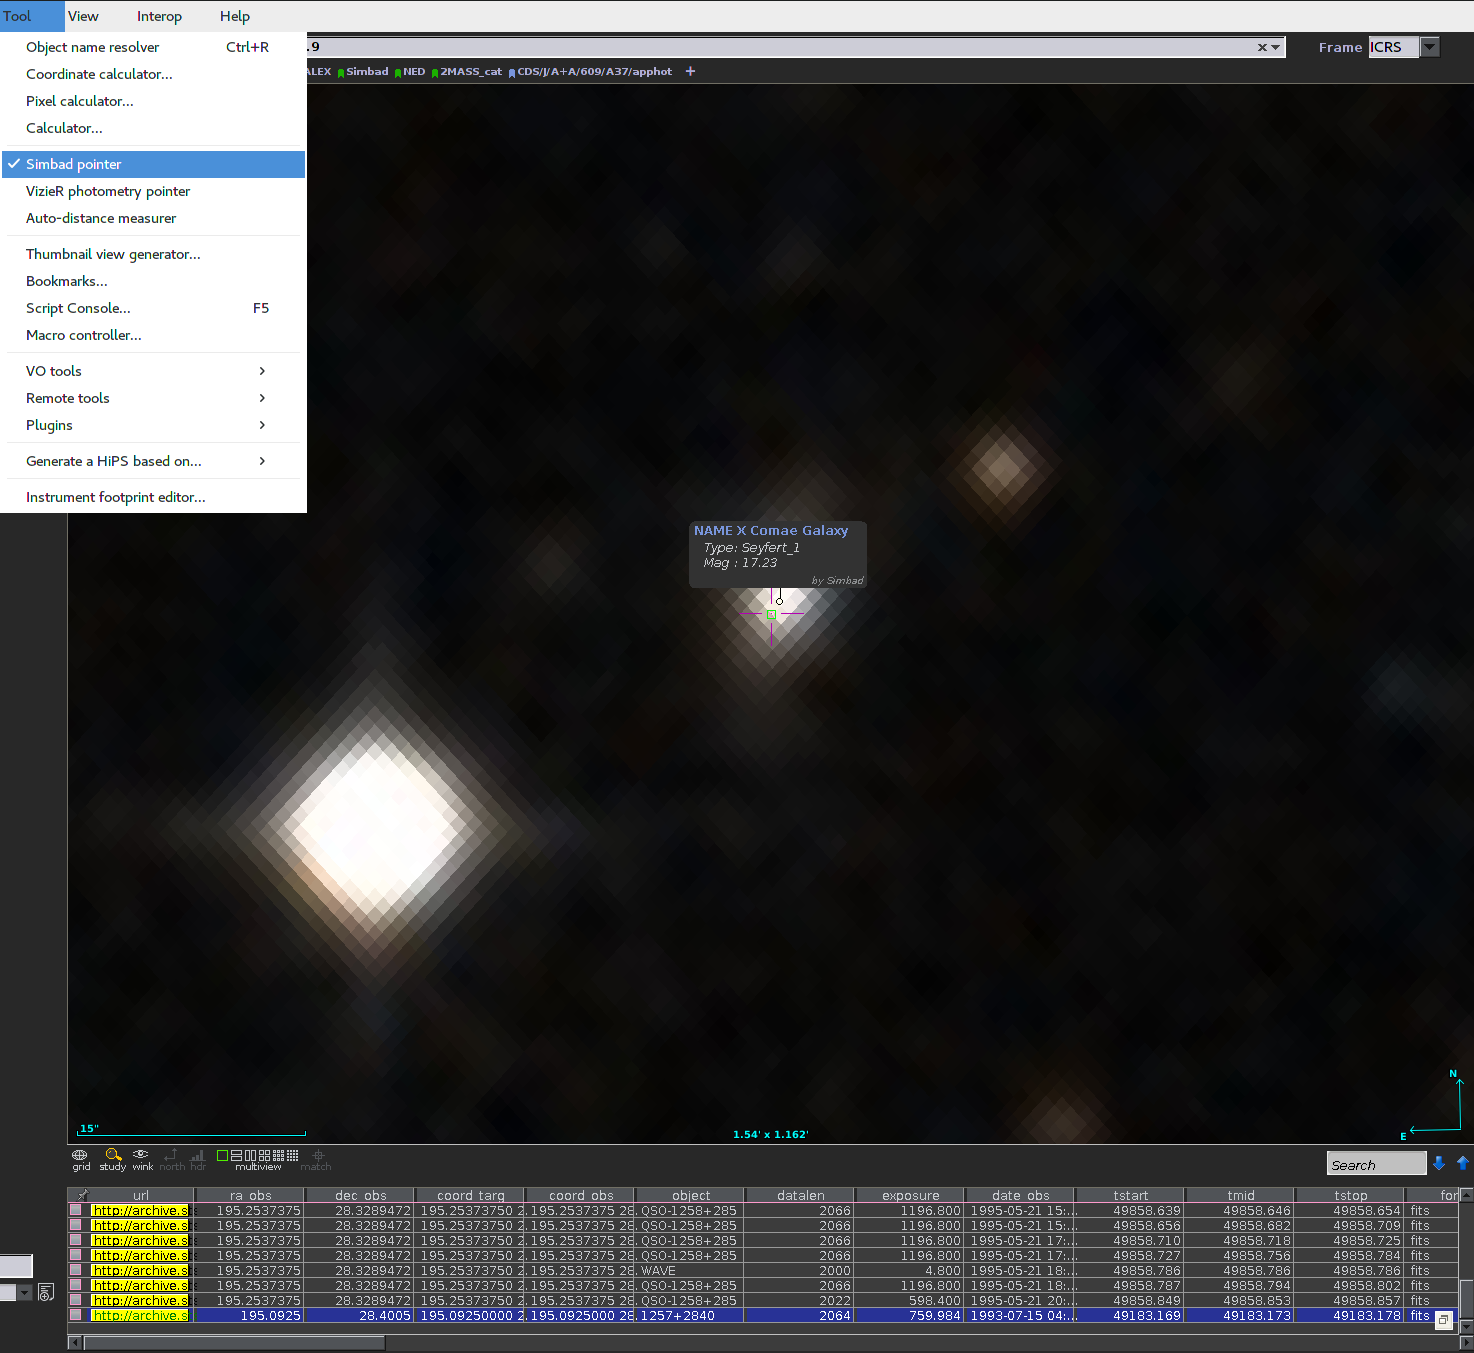
\includegraphics[width=0.5  
\textwidth]{../images/aladin_simbad_pointer-coma.png}
\caption{How to enable and operate the \simbad\ pointer in \aladin.}
\label{fig:slit}
\end{figure}
\item Clicking on the name of this galaxy (NAME X COMAE GALAXY) opens a web 
browser with all the \simbad\ information for this object. 
\item The radial velocity for this galaxy is 27332.1\,$\kms$. 
\item Note that this galaxy is not part of the Coma cluster since the velocity 
of the Coma cluster is 6845~$\kms$. This value can be found with \simbad\ 
looking for A1656. The hierarchical link 
\includegraphics[width=0.07 
\textwidth]{../images/simbad_button_parents.png} on NAME X COMAE GALAXY in 
\simbad\ confirms that the probability of this galaxy to belong to Coma is 0\%.
\end{itemize}

\item Go back to \cassis\ and change the \textbf{Vlsr plot} field from 0 to 
2.7e4\,$\kms$ (Figure~\ref{fig:spectrum3}). As soon as you click 
\textbf{Display} again, the green tick 
corresponding to the HI line moves right under the second fainter line in the 
HST spectrum. This confirms that this line is associated to this Seyfert 1 
galaxy.
\begin{figure}[H]
\center
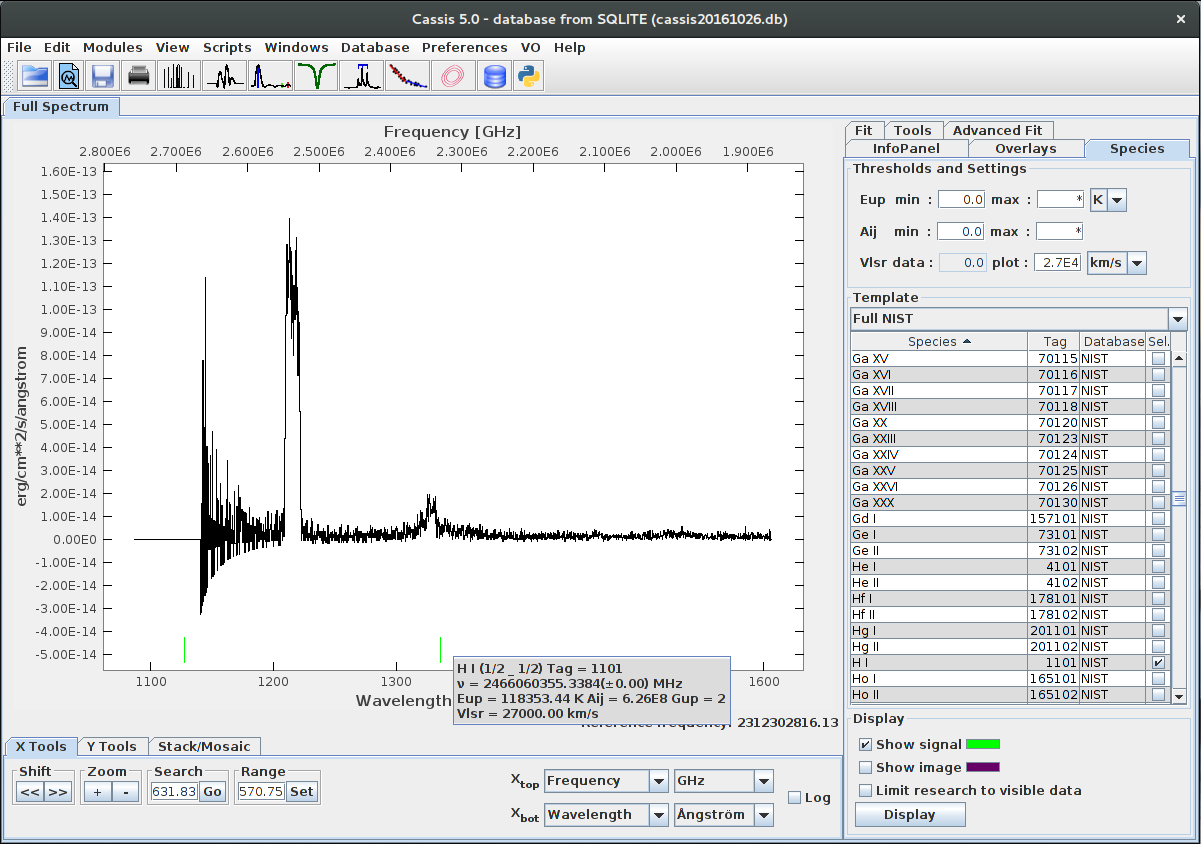
\includegraphics[width=0.6\textwidth]{../images/cassis_redshifted_line.png}
\caption{HI line of the Seyfert 1 galaxy.}
\label{fig:spectrum3}
\end{figure}
\end{itemize}

\section{Fit a gaussian and a continuum to the hydrogen line}

\begin{itemize}
\item Focus on a small portion of the spectrum, centred on the HI line of the 
Seyfert 1 galaxy and fit the line with a Gaussian profile and a continuum: In 
the \textbf{spectrum analysis} (if necessary open by clicking 
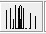
\includegraphics[width=0.05  
\textwidth]{../images/cassis_button_spec-analysis.jpg}) window, reduce the 
wavelength range: 
1300 to 1375 Angstr\"om and click 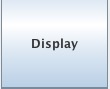
\includegraphics[width=0.05  
\textwidth]{../images/cassis_button_display.jpg}.
\item In the \cassis\ main window, select the \textbf{Fit} tab and add two 
components using the \textbf{Manage Components} menu: a polynomial baseline and 
a Gaussian line.
\item Change the \textbf{degree} of the polynomial to ` 0 ' in order to fit a constant baseline.
\item For the Gaussian component, the purple/blue fields should be filled with 
initial values in order to start the fitting procedure. They can be filled by 
hand but a useful way of filling them in is: use the middle button of your 
mouse to click and drag the region of the line or alternatively with a trackpad 
press both ctrl+alt and click and drag to draw the region. Beware that the 
Gaussian parameters should stay violet/blue (do not click on any of them) if 
you want them to fill in automatically. The position of the peak (\textbf{xo}), 
its height (\textbf{Io}) and the width of the line (\textbf{FWHM}) are 
estimated automatically from the selection. This selection, visible in 
purple/blue on Figure \ref{fig:specfit}, can be erased using the \textbf{reset} 
buttons in \textbf{Selections [with middle-click-and-drag]}.
\item Click on \textbf{Fit current} to perform a fit of the line+baseline. The different components of the fit can be selected or deselected in the \textbf{InfoPanel}.
\item Go back to the \textbf{Fit} panel and note the central wavelength of this line as inferred from the best fit: 1327 Angstr\"om. 
\begin{figure}[H]
\center
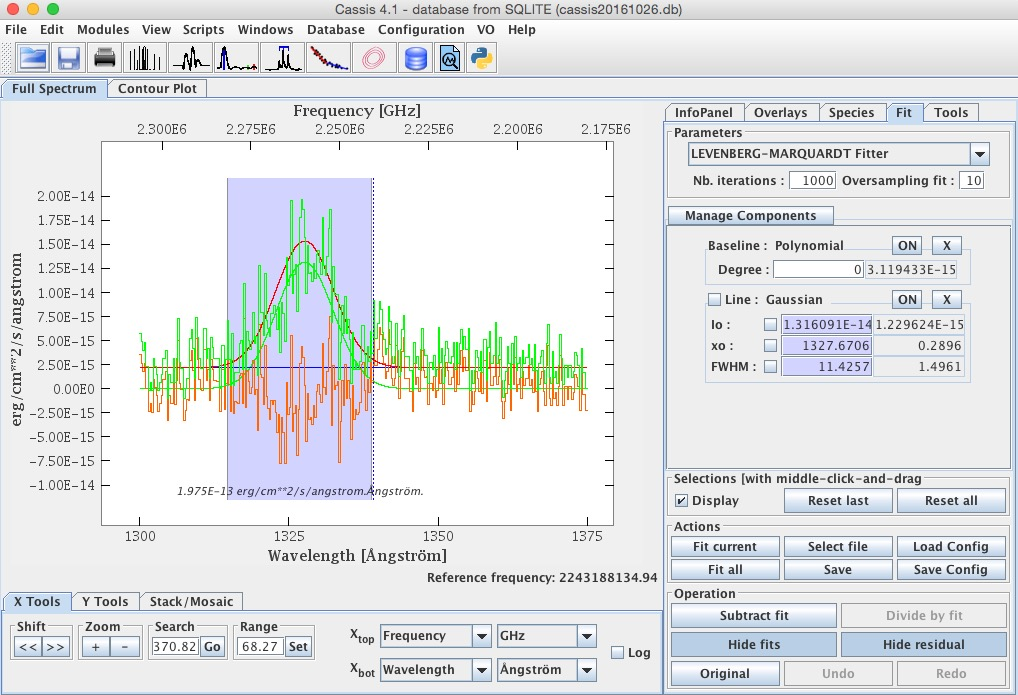
\includegraphics[width=0.6  \textwidth]{../images/cassis_window_fit-spec.jpg}
\caption{Fit of the spectrum.}
\label{fig:specfit}
\end{figure}
\item Given that the rest wavelength for the Lyman $\alpha$ line is 1215.67 Angstr\"om, the velocity of the galaxy is v=c$\times\Delta\lambda/\lambda_0$=27,420~$\kms$ or in redshift, z=v/c=0.0914.

\item This value can be compared to the value given in \simbad.
\end{itemize}
 
\section{Scripting in a Jupyter notebook [optional]}

The tasks in this tutorial can also be carried out using a Jupyter notebook. 
Go now to\\
\url{https://mybinder.org/v2/gh/kathl/VOtutorials_with_Python/master}\\
and wait a moment for everything to load. You should then see list of files. 
Click on the link to 

\textbf{Abel1656\_The\_Coma\_Cluster\_of\_Galaxies.ipynb}

\noindent and follow the instructions there. You can also download the Jupyter 
notebook from the github repository to your machine. It was created to run with 
the packages as listed in the requirements.txt file. Using 
pip\footnote{\url{https://pip.pypa.io/en/stable/}} you can install all these 
packages with the command \texttt{pip install [name of the package]}. 

%\bibliographystyle{unsrtnat} % Use the "unsrtnat" BibTeX style for formatting the Bibliography
%\bibliography{Bibliography}


\end{document}


